\documentclass{article}

\usepackage[spanish]{babel}
\usepackage{listings}
\usepackage{color}
\usepackage[numbers,sort&compress]{natbib}
\usepackage{graphicx}
\usepackage{subfigure}
\usepackage{url}
\usepackage{amsmath}
\usepackage{hyperref}
\usepackage[top=15mm, bottom=40mm, left=15mm, right=15mm]{geometry}
\setlength{\parskip}{2mm}
\setlength{\parindent}{0pt}

\setlength{\parskip}{2mm}
\setlength{\parindent}{0pt}
\definecolor{blue}{rgb}{0,0.6,0}
\definecolor{gray}{rgb}{0.3,0.3,0.3}
\definecolor{orange}{rgb}{0.8,0.4,0}
\definecolor{mostaza}{rgb}{0.9,0.8,0.1}

\lstset{ %
  language=R,                     % the language of the code
  basicstyle=\footnotesize,       % the size of the fonts that are used for the code
  numbers=left,                   % where to put the line-numbers
  numberstyle=\tiny\color{gray},  % the style that is used for the line-numbers
  stepnumber=1,                   % the step between two line-numbers. If it's 1, each line
                                  % will be numbered
  numbersep=5pt,                  % how far the line-numbers are from the code
  backgroundcolor=\color{white},  % choose the background color. You must add \usepackage{color}
  showspaces=false,               % show spaces adding particular underscores
  showstringspaces=false,         % underline spaces within strings
  showtabs=false,                 % show tabs within strings adding particular underscores
  frame=single,                   % adds a frame around the code
  rulecolor=\color{black},        % if not set, the frame-color may be changed on line-breaks within not-black text (e.g. commens (green here))
  tabsize=2,                      % sets default tabsize to 2 spaces
  captionpos=b,                   % sets the caption-position to bottom
  breaklines=true,                % sets automatic line breaking
  breakatwhitespace=false,        % sets if automatic breaks should only happen at whitespace
  title=\lstname,                 % show the filename of files included with \lstinputlisting;
                                  % also try caption instead of title
  keywordstyle=\color{orange},      % keyword style
  commentstyle=\color{blue},   % comment style
  stringstyle=\color{mostaza},      % string literal style
  escapeinside={\%*}{*)},         % if you want to add a comment within your code
  morekeywords={*,...}            % if you want to add more keywords to the set
} 

\author{1445183}
\title{Práctica 5: Método Monte-Carlo}
\date{\today}

\begin{document}

\maketitle

\section{Intoducción}
El método Monte-Carlo \cite{monte} permite calcular estadísticamente algún valor que no se conoce y que es díficil calcular analíticamente. 

\section{Objetivo}
Calcular el valor de la integral \eqref{fx} proporcionada por la práctica usando el método Monte-Carlo para la función \eqref{fx2}, teniendo como referencia el valor de la integral obtenido mediante Wolfram Alpha \cite{wa}. 
\begin{equation}
 \int_{3}^{7} f(x) d(x) 
\label{fx}
\
\end{equation}

\begin{equation}
f(x) = \frac{1}{exp(x) + exp(-x)}
\label{fx2}
\end{equation}


\section{Descripción}
Para la elaboración de la práctica se utilizó el código base proporcionado  \cite{elisaweb5}, al cual se le modificó el tamaño de muestra (pedazo) con 5 diferentes valores con 50 repeticiones cada uno, haciendo uso de \texttt{for} como se muestra en el código \texttt{R} siguiente:

\begin{lstlisting}[language=R]
for (pedazo in c(100,1000,10000,100000,1000000)) {
  print(paste("pedazo", pedazo))
  for (repeticiones in 1:50) {
    montecarlo <- foreach(i = 1:cuantos, .combine=c) %dopar% parte()
    integral <- sum(montecarlo) / (cuantos * pedazo)
    resultados <- (pi / 2) * integral
    diferencia <- (valor-resultados)
    vectores <- rbind(vectores, c(repeticiones, pedazo, valor, resultados, diferencia))
  }
}
\end{lstlisting}

\newpage
De esta manera se obtienen los valores de la integral para cada tamaño de muestra así como el error de cada uno, expresados en gráficas caja-bigote, para comparación de los resultados se toma en cuenta el valor de la integral obtenido mediante Wolfram Alpha \cite{wa}.

\section{Resultados}

Como se muestra en la figura \ref{figura 1} la aproximación al valor real \texttt{0.048834} de la integral (línea roja) es mayor conforme aumenta el tamaño de muestra lo que también afecta en el error, ya que este disminuye al aumentar el tamaño de muestra.

\begin{figure}[htbp]
\centering
\subfigure[]{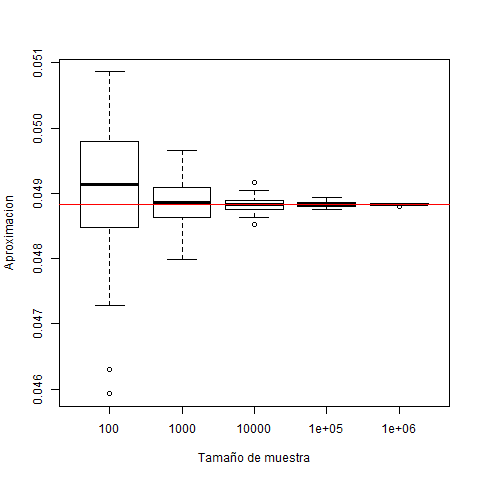
\includegraphics[width=80mm]{./p5a.png}}
\subfigure[]{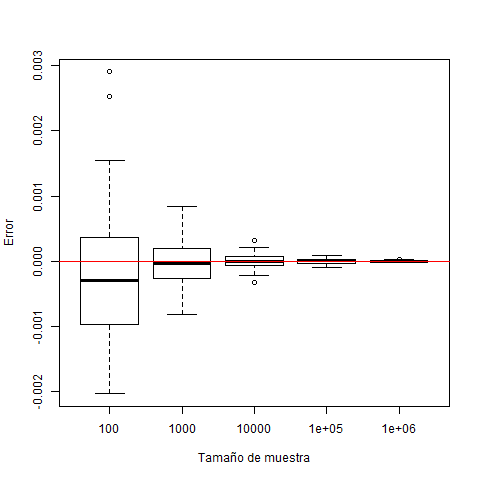
\includegraphics[width=80mm]{./p5e.png}}
\caption{Aproximación al valor real y error vs tamaño de muestra} \label{figura 1}
\end{figure}

En el cuadro \ref{esto} se puede ver que el tamaño de muestra con mayor valor es el que tiene mayor precisión en más lugares decimales y viceversa con el valor de referencia \texttt{0.048834}
\begin{table}[h!]
\caption{Comparación de decimales por tamaño de muestra}
\label{esto}
\vspace*{3mm}
\centering
\begin{tabular}{l|c|r} 
Tamaño de muestra & Valor aproximado & Error \\  \hline
100 & 0.04611858 & 0.000003597 \\
1000 &  0.04931986 & -0.0004858631 \\
10000 & 0.04864882 & 0.0001851811 \\
100000 & 0.04879861 & 0.00003538998 \\
1000000 & 0.04883115 & 0.000002852509 \\
\end{tabular}
\end{table}

\newpage

\section{Conclusiones}

Mediante el método Monte-Carlo se obtuvieron los valores aproximados al de referencia, para los valores asingados en este reporte el tamaño de muestra con valor de 1,000,000 (valor mayor utilizado) es el valor con más decimales de precisión con el de referencia y también es el valor con menor error. 
De manera que entre mayor sea el tamaño de muestra, es decir, los puntos dentro de la integral, la precisión de obtener el resultado correcto aumenta.

\bibliographystyle{plainnat}
\bibliography{bibliosimu}

\end{document}